\documentclass{aamas2015}
\usepackage{amsmath}

\pdfpagewidth=8.5truein
\pdfpageheight=11truein

\begin{document}

\title{Exploiting Object Symmetry for Efficient Grasping}
\numberofauthors{1}

\author{
\alignauthor
Paper XXX
}

\newcommand{\vech}[1]{\textbf{#1}}
\newcommand{\set}[1]{\textbf{#1}}

\maketitle

%% IDEAS
% - force map instead of collision map
% - invariance of height?
% - projection of fingers convex ?
% - add 3rd dimension (saturation)?
% - changing circle size by cutting through a cone. Allows for change in height.


\begin{abstract}
In this, paper we introduce an efficient representation for robot grasping that exploits symmetry
properties of objects. The new representation forms a low-dimensional manifold, which can be used to
identify the set of feasible grasps during a sequential manipulation task. We analyse the properties
of this low-dimensional manifold and show that some of these properties can be used for fast
manipulation planning. We apply the introduced representation and planner to bi-manual manipulation
in humanoid robots.
\end{abstract}

% representation (high level / abstract)
% manifold (2 dimensional thing)

\section{Introduction}
Robots with advanced dexterous capabilities have the potential
to revolutionize important application domains such as 
healthcare, security, or manufacturing. Whether it is in 
structured environments such as factories, or unstructured 
environments such as homes, grasping is often the first 
step in the physical interaction between a robot and 
its surroundings. The generation of grasps on objects 
is therefore at the heart of planning physical tasks.
However, to date, most grasp planning methods are mainly 
focused on generating physically stable grasps, without
incorporating immediate or future task constraints. 

Many well established algorithms assume only a single action, 
and do not include foresight and reasoning about next 
actions. However, when picking up a mug, it is 
important to select a grasp that facilitates
the next action to be performed. In case the next action 
is a pouring motion, the robot needs avoid grasps that would 
cover the rim of the object. In contrast, if any of the 
next actions involves placing the mug on the table, the 
robot cannot choose any grasp in which fingers touch 
the mug's base. To date, many grasp representations 
are based on a floating hand representing only the 
end-effector and ignoring the embodiment of the 
entire robot in environment. As a result, infeasible grasps 
are generated and have to be pruned out in a post-processing 
step. Yet, selecting grasps that facilitate task completion is 
particularly important for bi-manual, sequential, 
and co-worker scenarios. In these scenarios, grasps
need to be carefully chosen, such that they do not violate
constraints imposed by a second arm, a human interaction
partner, or a future action. 

In this paper, we address the issue of manipulation planning with task
constraints. We are particularly interested in tasks that involve several
subtasks or several interacting agents. Planning grasps for such 
tasks can rapidly become computationally infeasible due to a large
search space. The key insight of this paper is that re-occurring
patterns in the geometry of shapes can be exploited to drastically
reduce the space of solutions. We will introduce an low-dimensional, 
object-centered representation for grasp planning which is based on rotational symmetries.
The symmetric nature of the objects allows us to update our representation
as the object rotated around the axis of symmetry. \emph{Since the object is symmetric any stable grasp can be rotated around the axis yielding a family of feasible grasps}. We will show that this basic property leads to a significant reduction of search complexity in grasp planning. Specifically, this property allows us to generate multiple grasps around the object which is useful for bi-manual tasks and cooperative robot hand over tasks. In addition, it allows us to identify a single grasp that is useful for a sequence of tasks.



%
%	
%
%\item Advantages of approach?
%	\begin{enumerate}
%	\item 
%	
%\item Contributions?
%	\begin{enumerate}
%	\item new representation for efficient parameterization of stable grasps 	
%	\item discussion of properties of representation induced by symmetric objects
%	\item a grasp planning algorithms using representation to achieve sequential and 
%		  bimanual tasks  
%	\end{enumerate}
%	\end{enumerate}
%	
%	
%
%\begin{enumerate}
%\item What is paper about?
%	\begin{enumerate}
%	\item Robots are required for assisting in collaborative tasks
%	\item Especially physical taks, e.g., domestic environments, healthcare, 
%		  defense, manufacturing 
%	\item Robots need manipulation and grasping capabilities (one of most 
%		  important behaviors)
%	\item Grasping is at the heart of planning physical tasks 
%	\end{enumerate}
%
%\item What is the problem?
%	\begin{enumerate}
%	\item Grasp planning taking into account environment and task constraints
%	\item Current grasp representations are based on a floating hand, which only 					  represents the end-effector and ignores embodiment of whole robot in
%		  environment. As a result, infeasible grasps are generated and have to be
%		  pruned out in a post-processing step. 
%	\item Well established algorithms assume only one action, and do not include
%		  foresight and reasoning about next actions to perform. Example, pouring
%		  into a cup. Example, putting mug into washing machine.
%	\item Motion planning with multiple subtasks -> planning needs to be fast 
%		  as possible (complexity)
%	\item !Try to show that separation of planning and grasp selection is naive
%	\item Especially in bi-manual, sequential and co-worker scenarios, complexity increases
%	\end{enumerate}
%	
%\item What is our approach?
%	\begin{enumerate}
%	\item Reoccurring patterns in the geometry of shapes can be exploited
%	\item Rotational and linear symmetries and extrusions can be exploited
%	\item In this paper we focus on rotational symmetries
%	
%	\item Object-centered representation
%	\item Project world and hand information into the representation, thereby taking
%		  into account reachability and collisions
%	\item Examples, picture of symm. object with two hands and hands are projected 
%		  into manifold.
%	\item 
%\end{enumerate}
\section{Related Work}

\section{Manifold Representations \\for Rotationally Symmetric \\Objects}
In this section we will introduce a low-dimensional representation for grasp 
planning on rotationally symmetric objects. The main idea is to project
the surface of the object onto a two-dimensional manifold, where each
point on the manifold corresponds to a possible grasp of the robot. Planning
can then be performed by identifying a point on this manifold which fulfills
all task constraints.

\subsection{Cylindrical Parametrization of \\Surface Points}
The manifold representation which will be discussed in the remainder of the paper is based
on a cylindrical coordinate system. We will therefore start by introducing cylindrical
coordinates. 

\begin{figure}[h!]
  \begin{center}
    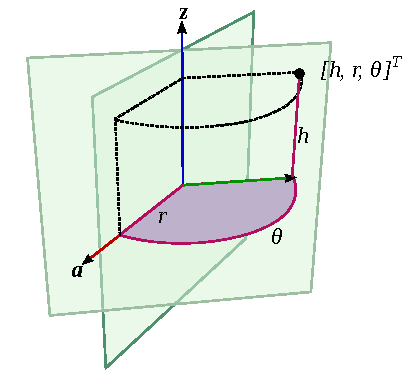
\includegraphics[width=0.4\textwidth]{./images/cylindricalCS.pdf} \quad
  \end{center}
  \caption{A cylindrical coordinate system used to parameterize points on the
  surface of a rotationally symmetric object. The axis $\vech{a}$ corresponds to the polar axis, while $\vech{h}$ is the axis of symmetry. Any point on the surface can be represented using height $h$, radius $r$, and angle $\theta$. \label{fig:cylindricalcs}}
\end{figure}
 
Let $\vech{z}$ be the axis of symmetry, $\vech{o}$ be the origin, and $\vech{a}$ be the polar axis of the object. The polar axis lies in the reference plane of the object and is perpendicular to $\vech{z}$. Subsequently, we assume that the reference plane is the base of object. Note that $\vech{a}$ can be arbitrarily chosen, since the object is symmetric. Using $\vech{z}$, $\vech{a}$ and their crossproduct we can form a local coordinate frame $L$ for an object. Any point $\vech{p} = [x,y,z]^T$ in the local coordinate frame $L$, can also be represented using a cylindrical parametrization of the coordinate system. This parametrization leads to a point $[h, r, \theta]^T$ whose components correspond to the height, radius and angle of the point respectively as seen in Fig.~\ref{fig:cylindricalcs}. The height is measured along the axis of symmetry $\vech{z}$, the radius $r$ is the distance between $\vech{p}$ and $\vech{z}$, the angle $\theta$ is the angle between $\vech{a}$ and the projection of $\vech{p} $ onto the local reference plane of the object as can be seen in Fig.~\ref{fig:cylindricalcs}. 

In the following, we define the radius as a function $r(h)$ of the height, which results in a two-dimensional parametrization $[h, \theta]^T \in \mathbb{S}$ of point $\vech{p}$. Subsequently, we can define the function $f: \mathbb{S} \rightarrow \mathbb{R}^3$ that maps the cylindrical coordinates to the 3D local coordinates in the following way:
		
		
\begin{equation}
	f(\vech{x}) = f([h, \theta]^T) = \left[ 
	\begin{array}{c}
	(h) ~ cos(\theta) \\ r(h) ~ sin(\theta)\\ h 
	\end{array} \right]. 
\end{equation}
		
Similarly, we can map from the 3D local coordinate space $L$ back to the 
surface manifold using the inverse mapping, $f^{-1}: \mathbb{R}^3 \rightarrow \mathbb{S}$:
\begin{equation}
	f^{-1}(\vech{p}) = f^{-1}([x,y,z]^T) = \left[ \begin{array}{c} z \\ atan2(y,x) \end{array}\right].
\end{equation}
The assumption of rotational symmetry along with the definition of the radius as a function of the height reduces the our parametrization to two variables. Fig.~\ref{} depicts the mapping of a 3D cylinder onto the 2D manifold. In the next section, we will see how this can exploited for generating grasps.

\begin{figure}[h!]
  \begin{center}
    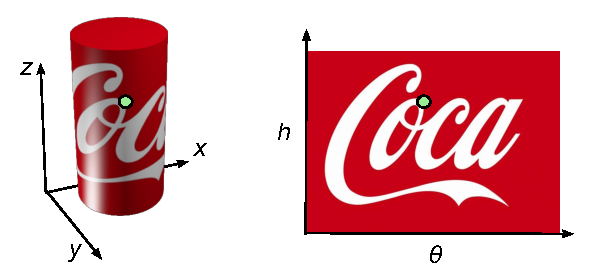
\includegraphics[width=0.45\textwidth]{./images/unfolding.pdf} \quad
  \end{center}
  \caption{The points on the 3D surface (right) are projected onto a two-dimensional manifold using a cylindrical coordinate system.\label{fig:unfolding}}
\end{figure}

\subsection{Grasp Manifold}
 In this section, we demonstrate how to exploit the introduced representation and the symmetry properties of the object to efficiently sample feasible grasps. The key insight is that stable grasps can be rotated around the axis of symmetry without having to modify the hand shape. We begin the analysis with a simplified grasping model where a point on the surface corresponds wrist position during grasping. The hand is assumed to be parallel to the base of the object such that the plane between the grasping fingers is perpendicular to the axis of symmetry. The goal is to identify the set of feasible points the robot can grasp. This requires reasoning about reachability and collisions, where we need to ensure that there is a collision-free arm pose with the wrist touching the respective surface point. To sample this space, we propose discretizing the manifold by fixed step sizes for the height $h$ and the angle $\theta$. Refer to picture. For each patch of the discretized manifold, using the center point  as the reference for the wrist, we attempt to compute a collision-free inverse kinematics solution. Refer to picture again showing red/blue and which collisions were caused. An interesting property of this representation is that the produced map can be efficiently updated when the object is rotated around its axis of symmetry. More specifically, a rotation around the z-axis corresponds to a shift along the $\theta$ dimension. 


% cyclic manifold 
\begin{enumerate}
	\item Define frames $L$ and $G$ as local object frame and global frame
	\begin{enumerate}
		\item 
		Let $\vech{z}$ be the axis of symmetry, $\vech{o}$ be the origin, and $\vech{a}$ be the polar axis of the object.The polar axis lies in the reference plane of the object and is perpendicular to $\vech{z}$. In the following, we assume that the reference plane is the base of object. Note that $\vech{a}$ can be arbitrarily chosen, since the object is symmetric. Using $\vech{z}$, $\vech{a}$ and their crossproduct we can form a local coordinate frame $L$ for an object.
		
		\item Any point $\vech{p} = [x,y,z]^T$ in the local coordinate frame $L$, can also be represented using a cylindrical parametrization of the coordinate system. 
		
		\item This parametrization leads to a point $[h, r, \theta]^T$ whose components correspond to the height, radius and angle respectively. The height is measured along the axis of symmetry $\vech{z}$, the radius $r$ is the distance between $\vech{p}$ and $\vech{z}$, the angle $\theta$ is the angle between $\vech{a}$ and the projection of $\vech{p} $ onto the local reference plane of the object as can be seen in Fig.~\ref{}. 
		
		\item In the following, we define the radius as a function $r(h)$ of the height, which leads to a two-dimensional parametrization $[h, \theta] \in \mathbb{S}$ of point $\vec{p}$. Subsequently, we can define the function $f: \mathbb{S} \rightarrow \mathbb{R}^3$ that maps the cylindrical coordinates to the 3D local coordinates in the following way:
		
		\begin{equation}
			f(\vech{x}) = f([h, \theta]) = [r(h) ~ cos(\theta), r(h) ~ sin(\theta), h]
		\end{equation}
		
		\item Similarly, we can map from the 3D local coordinate space $L$ to the 
		surface manifold using the inverse mapping, $f^{-1}: \mathbb{R}^3 \rightarrow \mathbb{S}$:
		
		\begin{equation}
			f^{-1}(\vech{p}) = f^{-1}([x,y,z]) = [z, atan2(y,x)]
		\end{equation}
		
		\item Wrap up: Having defined the forward and backward mappings, now we can discuss how this is useful.
	\end{enumerate}
	
	\item Parametrizing Grasps using Low Dimensional Manifolds
	\begin{enumerate}
		
		\item In this section, we demonstrate how to exploit the introduced representation and the symmetry properties of the object to efficiently sample feasible grasps. The key insight is that stable grasps can be rotated around the axis of symmetry without having to modify the hand shape. 
			
		\item We begin the analysis with a simplified grasping model where a point
		on the surface corresponds wrist position during grasping. The hand is assumed to be parallel to the base of the object such that the plane between the grasping fingers is perpendicular to the axis of symmetry. 

		\item The goal is to identify the set of feasible points the robot can grasp. This requires reasoning about reachability and collisions, where we need to ensure that there is a collision-free arm pose with the wrist touching the respective surface point. To sample this space, we propose discretizing the manifold by fixed step sizes for the height $h$ and the angle $\theta$. Refer to picture.
		
		\item For each patch of the discretized manifold, using the center point 
		as the reference for the wrist, we attempt to compute a collision-free 		inverse kinematics solution. Refer to picture again showing red/blue and which collisions were caused. 
		
		\item An interesting property of this representation is that the produced map can be efficiently updated when the object is rotated around its axis of symmetry. More specifically, a rotation around the z-axis corresponds to a shift along the $\theta$ dimension. 
		
		\item 
	\end{enumerate}
	
	\item Low-dimensional manifold for grasps on symmetric objects	
	\begin{enumerate}
	\item Let $\vech{x} \in \set{S}, where \vech{x} = [h, \theta]^T$
	\item $h$ is the height of the contact point along the axis of symmetry
	\item $r$
	\end{enumerate}

\end{enumerate}

% name it!
% unwrapping introduces a nonlinear warping
%

% symmetry and invariance
% Pic1: wiki cylinder parameterization
% Pic2: coke picture
% Pic3: discretization and red/blue stuff with bottle
% Pic4: multiple hand rotations around object (wine bottle)
% Pic5: project robotiq hand onto coke

\section{Task Planning with Grasp Manifolds}
% Pic5: two tasks superimposed on top of each other (manifold pictures and simulation) and one object rotating

 
\subsection{Planning for Task Sequences}
% Pic6: Rod through 3 tasks (superimposed)

\subsection{Planning for Bi-Manual and Cooperative Tasks}
% Pic7: Hand prints of two robots (two different robot hands, robotiq vs. tweezer)
% Pic8: Picture of two robots in front of each other, hand over

\section{Experiments}
% offline experiment: how fast is map generation? 
% online experiment: how fast is sequence generation?
% quality? how good? alternative solutions?
% Pic8: 3D blob
% 2 different domains
 
\section{Discussion}
% this representation introduces warping effects
% talk about variable radius objects (picture)
% hierarchical grid, importance, details lost
% using profile instead of height
\section{Conclusions}

\end{document}
